\chapter{Спин, изоспин, цвет и самодействие глюонов}

\section{Квантовая хромодинамика по аналогии с электродинамикой}

Квантовая хромодинамика — слишком обширная тема, чтобы полностью изложить её в одной лекции. Цель здесь — основная интуитивная картина, а не более глубокая математика.

Квантовая электродинамика — это теория электронов и фотонов. Она также является квантовой теорией кулоновской силы. Если рассматривать ядро атома как фиксированный источник электрического поля, не задаваясь вопросами о его движении или внутренней структуре, то КЭД является теорией атома.

Квантовая хромодинамика играет аналогичную роль для кварков и глюонов. Она описывает сами частицы, силы между ними и составные объекты, которые они образуют. Эти составные объекты называются \emph{адронами}. Протоны и нейтроны — это барионы: они несут суммарное кварковое число, или, эквивалентно, ненулевое барионное число. Мезоны — это комбинации кварк--антикварк. И барионы, и мезоны также содержат глюоны.

Глюоны электрически нейтральны, но именно они обеспечивают поле, которое связывает кварки. В этом отношении глюонное поле играет роль, аналогичную электромагнитному полю, которое связывает атомы.

Прежде чем вводить цвет и глюоны, полезно вернуться к математике спина. Та же математика почти непосредственно возникает снова как \emph{изоспин}, а родственная схема ещё раз появляется в теории цвета. В основе этих построений лежит теория групп, но необходимые идеи можно развить через момент импульса.

\section{Мультиплеты момента импульса}

Компоненты момента импульса удовлетворяют соотношению
\begin{equation}
[L_x,L_y]=i\hbar L_z,
\end{equation}
вместе с циклически связанными с ним соотношениями
\begin{equation}
[L_y,L_z]=i\hbar L_x,
\qquad
[L_z,L_x]=i\hbar L_y.
\end{equation}
Эти три компоненты не коммутируют, поэтому все они не могут быть измерены одновременно. Поэтому в описании выделяют одну ось, по соглашению ось \(z\), и обозначают состояния компонентой момента импульса вдоль этой оси.

Этот выбор не нарушает вращательную симметрию в природе. Он нарушает симметрию только в описании, выделяя одно направление для учёта.

Допустимые значения \(z\)-компоненты квантованы и отличаются на одну единицу \(\hbar\). Полагая \(\hbar=1\) при перечислении этих значений, получаем, что мультиплет спина \(\ell\) содержит
\begin{equation}
m=\ell,\ell-1,\ldots,-\ell.
\end{equation}
Следовательно, число независимых состояний равно
\begin{equation}
2\ell+1.
\end{equation}

Первые несколько мультиплетов стоит выписать явно:
\begin{align}
\ell=0:&\qquad m=0,\\
\ell=\frac12:&\qquad m=\frac12,-\frac12,\\
\ell=1:&\qquad m=1,0,-1,\\
\ell=\frac32:&\qquad
m=\frac32,\frac12,-\frac12,-\frac32,\\
\ell=2:&\qquad m=2,1,0,-1,-2.
\end{align}

Для наших целей полуцелый спин относится к фермионам, а целый — к бозонам. Электрон — частица со спином \(\tfrac12\). Частица с нулевым спином вообще не имеет момента импульса. Фотон имеет спин, равный единице, и состояния со спином единица встречаются также у атомов и ядер. Атомы и ядра могут также иметь спин \(\tfrac32\), и тот же подсчёт продолжается и для больших значений спина.

В обозначениях нужно различать полный спин и его компоненту. Число \(\ell\) обозначает мультиплет и одновременно является максимально возможной \(z\)-компонентой. Число \(m\) обозначает конкретное состояние внутри этого мультиплета. Поэтому объект со спином единица имеет три состояния, тогда как объект со спином \(\tfrac12\) имеет два.

\section{Сложение двух частиц со спином одна вторая}

Рассмотрим две частицы со спином \(\tfrac12\) и пренебрежём их орбитальным моментом импульса. Пространство произведения их спиновых состояний содержит четыре базисных состояния:
\begin{equation}
|\uparrow\uparrow\rangle,\qquad
|\uparrow\downarrow\rangle,\qquad
|\downarrow\uparrow\rangle,\qquad
|\downarrow\downarrow\rangle.
\end{equation}
Соответствующие \(z\)-компоненты равны
\begin{align}
|\uparrow\uparrow\rangle &: m=+1,\\
|\uparrow\downarrow\rangle &: m=0,\\
|\downarrow\uparrow\rangle &: m=0,\\
|\downarrow\downarrow\rangle &: m=-1.
\end{align}

Состояние, в котором оба спина направлены вверх, показывает, что мультиплет со спином единица обязательно присутствует: максимальная \(z\)-компонента равна \(+1\). Мультиплет со спином единица содержит только три состояния,
\begin{equation}
m=+1,\quad 0,\quad -1.
\end{equation}
Однако пространство произведения содержит четыре состояния, включая два независимых состояния с \(m=0\). Все они не могут принадлежать одному мультиплету со спином единица. Лишнее состояние не может иметь спин два, потому что мультиплет со спином два потребовал бы пять состояний. Следовательно, четыре состояния произведения должны разделиться на три состояния со спином единица и одно состояние со спином нуль.

Какая комбинация двух базисных состояний с \(m=0\) принадлежит мультиплету со спином единица? Переставим две частицы местами. Состояния с одинаково направленными спинами не изменяются:
\begin{equation}
|\uparrow\uparrow\rangle\longrightarrow|\uparrow\uparrow\rangle,
\qquad
|\downarrow\downarrow\rangle\longrightarrow|\downarrow\downarrow\rangle.
\end{equation}
Напротив, состояния произведения со смешанными спинами переходят друг в друга:
\begin{equation}
|\uparrow\downarrow\rangle
\longleftrightarrow
|\downarrow\uparrow\rangle.
\end{equation}
Их сумма симметрична относительно этой перестановки:
\begin{equation}
|\uparrow\downarrow\rangle+|\downarrow\uparrow\rangle.
\end{equation}
Нормировка даёт множитель \(1/\sqrt2\):
\begin{equation}
|1,0\rangle
=
\frac{|\uparrow\downarrow\rangle
      +|\downarrow\uparrow\rangle}{\sqrt2}.
\end{equation}

\begin{figure}[h]
\centering
\includegraphics[width=0.78\textwidth]{lecture_02_figure_02.png}
\caption{Симметричная комбинация состояний со смешанными спинами, образующая состояние \(m=0\) триплета со спином единица.}
\lectureframe{00:15:08}
\end{figure}

Вместе с двумя состояниями с одинаково направленными спинами это даёт триплет со спином единица:
\begin{align}
|1,+1\rangle &=|\uparrow\uparrow\rangle,\\
|1,0\rangle &=
\frac{|\uparrow\downarrow\rangle
      +|\downarrow\uparrow\rangle}{\sqrt2},\\
|1,-1\rangle &=|\downarrow\downarrow\rangle.
\end{align}
Оставшаяся ортогональная комбинация содержит знак минус:
\begin{equation}
|0,0\rangle
=
\frac{|\uparrow\downarrow\rangle
      -|\downarrow\uparrow\rangle}{\sqrt2}.
\end{equation}
Она антисимметрична относительно перестановки и образует односостоячный мультиплет со спином нуль. Итак,
\begin{equation}
\frac12\otimes\frac12=1\oplus0.
\end{equation}

Симметричное состояние со смешанными спинами имеет \(m=0\), но его полный момент импульса \emph{не} равен нулю. Оно принадлежит триплету со спином единица. При повороте координатной оси оно смешивается с состояниями \(m=\pm1\). Только антисимметричная комбинация имеет \(\ell=0\).

С точки зрения момента импульса синглет подобен пустому пространству. Он может нести энергию, заряд или другие квантовые числа, но момента импульса не несёт.

Это различие можно проверить мысленным экспериментом. Пренебрегите всеми законами сохранения, кроме закона сохранения момента импульса, и спросите, какое двухчастичное спиновое состояние могло бы просто исчезнуть. Ни одно из состояний с одинаково направленными спинами исчезнуть не могло бы, потому что каждое из них принадлежит мультиплету со спином единица. Симметричное состояние \(m=0\) тоже не могло бы исчезнуть. Хотя его \(z\)-компонента обращается в нуль, его полный спин по-прежнему равен единице и имеет нетривиальные компоненты относительно других осей. Без нарушения закона сохранения момента импульса исчезнуть мог бы только антисимметричный синглет.

\begin{classroomqa}
\audiencequestion{Дало бы измерение симметричного состояния со смешанными спинами вдоль оси \(z\) значение \(+1\) или \(-1\)?\lecturetimestamp{00:19:28}}
\lecturerresponse{Нет. Вдоль оси \(z\) оно даёт нуль. Тем не менее это состояние имеет полный спин, равный единице, поэтому измерение вдоль другой оси может дать \(+1\) или \(-1\).}
\end{classroomqa}

\section{Три частицы со спином одна вторая}

Теперь объединим три частицы со спином \(\tfrac12\). Имеется
\begin{equation}
2\times2\times2=8
\end{equation}
состояний произведения. Если все три спина направлены вверх, полная \(z\)-компонента равна \(+\tfrac32\). Следовательно, должен присутствовать мультиплет со спином \(\tfrac32\). Он содержит
\begin{equation}
2\left(\frac32\right)+1=4
\end{equation}
состояния.

Остаются четыре состояния. Они не могут образовать второй мультиплет со спином \(\tfrac32\), потому что состояния с \(m=\pm\tfrac32\) уже использованы. У оставшихся состояний максимальные компоненты равны лишь \(+\tfrac12\) и \(-\tfrac12\). И три полуцелых спина также не могут дать полный спин нуль. Оставшиеся состояния должны образовать мультиплеты со спином \(\tfrac12\).

Мультиплет со спином \(\tfrac12\) содержит два состояния. Поскольку остаются четыре состояния, существуют два различных мультиплета со спином \(\tfrac12\):
\begin{equation}
\frac12\otimes\frac12\otimes\frac12
=
\frac32\oplus\frac12\oplus\frac12.
\end{equation}
Эта схема появится снова, когда два состояния, называемые спином вверх и спином вниз, будут заменены двумя ароматами кварков, называемыми верхним и нижним.

\section{Изоспин как внутренний спин}

Изоспин, или изотопический спин, является внутренним аналогом обычного спина. Обычный спин связан с вращениями физического пространства. Изоспин — нет. Он относится к преобразованиям во внутреннем математическом пространстве, два базисных состояния которого будут отождествлены с
\begin{equation}
u,\qquad d.
\end{equation}
Термины \emph{верхний} и \emph{нижний} здесь являются лишь метками аромата. В обычном пространстве ничто не направлено ни вверх, ни вниз.

\editorialnote{Краткий переход между определением внутреннего спинового пространства и последующим рассуждением о масштабах масс адронов не удаётся уверенно восстановить. Из него не выводится никакого дополнительного физического утверждения.}

Почему \(u\) и \(d\) подходят для этой аналогии? Естественный энергетический масштаб адронной физики составляет несколько сотен МэВ. Типичный лёгкий мезон имеет массу в несколько сотен МэВ, и энергия, связанная со связыванием трёх кварков в нуклон, также имеет этот масштаб. Для сравнения, энергии связи обычных ядер составляют лишь несколько МэВ. Поэтому силу, удерживающую протоны и нейтроны вместе внутри ядра, рассматривают на гораздо меньшем энергетическом масштабе, чем динамику, связывающую кварки внутри адрона.

Среди шести ароматов кварков \(u\) и \(d\) легки по сравнению с адронным масштабом. Для рождения тяжёлых кварков требуется больше энергии, и адроны, содержащие их, могут распадаться на более лёгкие. Поэтому наиболее стабильные лёгкие адроны состоят из верхних и нижних кварков.

Нижний кварк тяжелее верхнего примерно вдвое в используемых здесь оценках, но обе массы малы по сравнению с сотнями МэВ. В первом приближении оба можно считать почти безмассовыми на адронном масштабе. Что ещё важнее, их можно считать почти равными по массе.

Это приближённое равенство приводит к симметрии. Если поменять местами верхний и нижний кварки, физика сильного взаимодействия меняется очень мало. Протон,
\begin{equation}
p\sim uud,
\end{equation}
и нейтрон,
\begin{equation}
n\sim udd,
\end{equation}
дают простейший пример: они отличаются перестановкой \(u\) и \(d\), и их массы очень близки.

Поэтому обмен
\begin{equation}
u\longleftrightarrow d
\end{equation}
математически рассматривается так же, как
\begin{equation}
|\uparrow\rangle\longleftrightarrow|\downarrow\rangle.
\end{equation}
Для обычного спина это преобразование соответствует повороту оси в пространстве. Для изоспина это поворот во внутреннем пространстве. Математика аналогична, хотя физический смысл различен.

\begin{figure}[h]
\centering
\includegraphics[width=0.80\textwidth]{lecture_02_figure_03.png}
\caption{Разложение двух состояний со спином \(\tfrac12\) на триплет и синглет — модель для соответствующего построения изоспина.}
\lectureframe{00:27:42}
\end{figure}

Префикс \emph{изо} происходит от \emph{изотоп}. В более раннем ядерном описании протон и нейтрон рассматривались как два члена одного внутреннего дублета. Обмен протона и нейтрона в ядре превращает один изотоп в другой. Позднее кварковая модель свела этот обмен протона и нейтрона к лежащему в основе обмену \(u\) и \(d\).

\begin{classroomqa}
\audiencequestion{Появилось ли понятие изоспина раньше кварковой модели?\lecturetimestamp{00:30:19}}
\lecturerresponse{Да. Изоспин был введён до появления кварков и исторически связан с Гейзенбергом. Кварковая модель позднее дала ему интерпретацию в терминах \(u\)- и \(d\)-ароматов.}
\end{classroomqa}

Изоспин не является точной симметрией природы. u- и d-кварки не имеют в точности равных масс, и их электрические заряды различны:
\begin{equation}
Q(u)=+\frac23,
\qquad
Q(d)=-\frac13.
\end{equation}
Даже если бы их массы были равны, электромагнетизм всё равно различал бы их.

Для малых адронных и ядерных систем электромагнитные эффекты слабы по сравнению с сильным взаимодействием. В большом ядре электрическое отталкивание может стать существенным; для протона, нейтрона или малого ядра, такого как гелий, это сравнительно малая поправка к масштабу сильного взаимодействия. Поэтому приближение изоспина состоит из двух шагов:

\begin{enumerate}
\item пренебречь различием масс \(u\)--\(d\);
\item отключить их электромагнитное различие и оставить только сильное взаимодействие.
\end{enumerate}

В рамках этого приближения преобразование между \(u\) и \(d\) становится симметрией, математически аналогичной обычной спиновой симметрии.

\section{Изоспиновый дублет нуклона}

Одиночный кварк нельзя изолировать и исследовать как свободный объект в лаборатории. Самые простые наблюдаемые барионы содержат три кварка. Поэтому аргумент подсчёта для трёх спинов имеет прямой аналог для изоспина: три кварка с изоспином \(\tfrac12\) могут образовать суммарный изоспин \(\tfrac32\) или \(\tfrac12\).

Начнём с полного изоспина \(\tfrac12\). Такой мультиплет содержит
\begin{equation}
2\left(\frac12\right)+1=2
\end{equation}
состояния. Это протон и нейтрон:
\begin{equation}
p\sim uud,
\qquad
n\sim udd.
\end{equation}
Их заряды равны
\begin{align}
Q(p)
&=\frac23+\frac23-\frac13
=+1,\\
Q(n)
&=\frac23-\frac13-\frac13
=0.
\end{align}
При перестановке \(u\) и \(d\) протон и нейтрон переходят друг в друга. Они образуют дублет с изоспином \(\tfrac12\).

Чтобы обсудить обменную симметрию, временно пометим три кварковых слота метками \(1,2,3\). Эти метки не следует принимать за фиксированные положения кварков; кварки движутся. Схематический множитель для протона имеет вид
\begin{equation}
d_1\bigl(u_2u_3-u_3u_2\bigr).
\end{equation}

\begin{figure}[h]
\centering
\includegraphics[width=0.58\textwidth]{lecture_02_figure_04.png}
\caption{Антисимметризованный множитель из двух \(u\)-кварков в схематическом состоянии протона.}
\lectureframe{00:35:43}
\end{figure}

Цель этого выражения — подчеркнуть фермионную антисимметрию при обмене. Это не полная волновая функция протона. Полное состояние должно объединять аромат, обычный спин, пространственную зависимость и---как вскоре окажется существенно важным---цвет.

\editorialnote{Нижние индексы — это временные метки слотов или одночастичных состояний. Два одинаковых состояния аромата \(u\) не образуют обычного антисимметричного изоспинового синглета, поэтому сам по себе показанный множитель не даёт оснований заключать, что изоспин равен нулю. Он сохранён лишь как локальный шаг антисимметризации по слотам; полный изоспин протона следует из его полного трёхкваркового состояния.}

Ограниченное сходство с более ранним построением для спина состоит в том, что квантовые состояния можно комбинировать симметрично или антисимметрично при обмене меток. Одно лишь это сходство не определяет изоспин, соответствующий показанному множителю \(uu\).

Протон обладает как обычным спином \(\tfrac12\), так и изоспином \(\tfrac12\). То же верно и для нейтрона. Это разные квантовые числа: обычный спин относится к физическим вращениям, тогда как изоспин относится к внутренней симметрии \(u\)--\(d\).

\section{Дельта-квартет}

Три лёгких кварка могут также образовывать полный изоспин \(\tfrac32\). Возникающий мультиплет из четырёх состояний — это дельта-квартет:
\begin{equation}
\begin{aligned}
\Delta^{++}&\sim uuu,
&
\Delta^{+}&\sim uud,
\\
\Delta^{0}&\sim udd,
&
\Delta^{-}&\sim ddd.
\end{aligned}
\end{equation}
Дельта-состояния обладают обычным спином \(\tfrac32\), а также изоспином \(\tfrac32\). В состояниях с максимальными компонентами все три обычных спина сонаправлены, и все три изоспина сонаправлены.

Состав вроде \(uud\) сам по себе не определяет, является ли состояние протоном или \(\Delta^+\). Один и тот же кварковый состав по ароматам можно скомбинировать в состояния с различными значениями полного спина и полного изоспина.

\begin{classroomqa}
\audiencequestion{Чем состояние \(uud\) из квартета Дельта отличается от протона?\lecturetimestamp{00:41:08}}
\lecturerresponse{Их обычные спины различаются. У протона спин \(\tfrac12\), тогда как у состояния Дельта спин \(\tfrac32\). Кварки также объединены в состояния с разным полным изоспином.}
\end{classroomqa}

\begin{classroomqa}
\audiencequestion{Являются ли средние члены квартета Дельта состояниями с изоспином \(\tfrac12\)?\lecturetimestamp{00:41:52}}
\lecturerresponse{Нет. Их проекции изоспина равны \(+\tfrac12\) и \(-\tfrac12\), но полный изоспин равен \(\tfrac32\). Мультиплет с полным изоспином \(\tfrac32\) неизбежно содержит четыре компонентных состояния.}
\end{classroomqa}

Четырём проекциям изоспина соответствуют
\begin{equation}
I_3=\frac32,\frac12,-\frac12,-\frac32.
\end{equation}
Их электрические заряды равны
\begin{align}
Q(\Delta^{++})&=+2,\\
Q(\Delta^{+})&=+1,\\
Q(\Delta^{0})&=0,\\
Q(\Delta^{-})&=-1.
\end{align}
Заряды двух средних состояний случайно совпадают с зарядами протона и нейтрона, но сами состояния остаются различными, поскольку их схемы сложения спина и изоспина различны.

Приближённая изоспиновая симметрия делает массы четырёх состояний Дельта почти равными. Небольшая разность масс кварков \(u\)--\(d\) вызывает лишь небольшое расщепление внутри квартета. Характерная масса состояний Дельта примерно равна
\begin{equation}
m_\Delta\sim1200\,\mathrm{MeV},
\end{equation}
тогда как массы протона и нейтрона близки к
\begin{equation}
m_N\sim940\,\mathrm{MeV}.
\end{equation}

\subsection{Распад \texorpdfstring{\(\Delta^{++}\)}{Delta++}}

Состояния Дельта достаточно тяжелы, чтобы распадаться на нуклон и пион. Рассмотрим
\begin{equation}
\Delta^{++}\sim uuu.
\end{equation}
По мере разлёта составляющих может родиться кварк--антикварковая пара. Попытка вставить \(u\bar u\) оставила бы в конечном состоянии барион из трёх \(u\) и не дала бы более лёгкого разрешённого канала при имеющейся энергии. Вместо этого рождение пары \(d\bar d\) позволяет перегруппировать составляющие как
\begin{equation}
uuu+d\bar d
\longrightarrow
uud+u\bar d.
\end{equation}
Два конечных составных состояния имеют вид
\begin{equation}
uud=p,
\qquad
u\bar d=\pi^+,
\end{equation}
поэтому
\begin{equation}
\Delta^{++}\longrightarrow p+\pi^+.
\end{equation}

\begin{figure}[h]
\centering
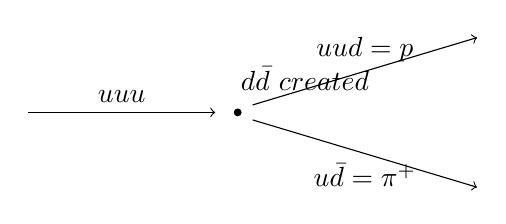
\begin{tikzpicture}[scale=0.95]
\draw[->] (-3,0) -- (-0.5,0) node[midway,above] {$uuu$};
\fill (-0.2,0) circle (1.5pt);
\draw[->] (0,0.1) -- (3,1.0) node[midway,above] {$uud=p$};
\draw[->] (0,-0.1) -- (3,-1.0) node[midway,below] {$u\bar d=\pi^+$};
\node at (0.7,0.45) {$d\bar d\ \text{created}$};
\end{tikzpicture}
\caption{Перегруппировка составляющих при распаде \(\Delta^{++}\rightarrow p+\pi^+\).}
\end{figure}

Сохранение заряда видно сразу:
\begin{equation}
Q(p)+Q(\pi^+)=1+1=2=Q(\Delta^{++}).
\end{equation}
Грубый баланс масс также допускает этот распад:
\begin{equation}
1200\,\mathrm{MeV}
>
940\,\mathrm{MeV}+140\,\mathrm{MeV}.
\end{equation}
Остаётся достаточно энергии, чтобы обеспечить кинетическую энергию конечного состояния.

Все четыре состояния Дельта могут распадаться на протон или нейтрон вместе с пионом. Их времена жизни чрезвычайно малы. Оценка по порядку величины — это время, за которое свет проходит поперёк протона:
\begin{equation}
\tau_\Delta
\sim
\frac{10^{-13}\,\mathrm{cm}}
     {10^{10}\,\mathrm{cm/s}}
\sim10^{-23}\,\mathrm{s}.
\end{equation}
Тем не менее они живут достаточно долго, чтобы их можно было идентифицировать как отдельные объекты, рождающиеся при столкновениях частиц.

\begin{classroomqa}
\audiencequestion{Имеет ли значение порядок, в котором записаны символы \(u\) и \(d\), в этом учёте составляющих?\lecturetimestamp{00:48:49}}
\lecturerresponse{Для рассматриваемой цели — нет. Важна информация об ароматовом составе и о том, как скомбинировано полное квантовое состояние.}
\end{classroomqa}

\section{Загадка Паули и необходимость цвета}

\(\Delta^{++}\) выявляет противоречие. Он состоит из трёх up-кварков. В состоянии со спином \(\tfrac32\) их обычные спины могут быть направлены в одну и ту же сторону. Их изоспины тоже одинаковы, потому что все они — \(u\). Если бы полное описание исчерпывалось спином, ароматом и пространственным состоянием с наименьшей энергией, то эти три кварка были бы тождественными фермионами, занимающими одно и то же состояние. Принцип запрета Паули это запрещает.

\begin{classroomqa}
\audiencequestion{Как несколько одинаковых up-кварков могут быть фермионами, если кажется, что они занимают одно и то же состояние?\lecturetimestamp{00:48:58}}
\lecturerresponse{Они не могут быть одинаковыми по всем квантовым числам. \(\Delta^{++}\) показывает, что кваркам нужна дополнительная метка помимо обычного спина, аромата и пространственного состояния. Эта дополнительная метка — цвет.}
\end{classroomqa}

Новая метка может принимать три возможных значения:
\begin{equation}
r,\qquad g,\qquad b,
\end{equation}
которые называют красным, зелёным и синим. Эти слова не имеют никакого отношения к видимому цвету. Это произвольные названия трёх внутренних состояний. Можно было бы использовать и другие названия; важно лишь то, что есть три различные возможности.

Красный, зелёный и синий варианты кварка данного аромата имеют одну и ту же массу и одни и те же обычные наблюдаемые свойства. Тем не менее это разные квантовые состояния. Поэтому \(\Delta^{++}\) может содержать один красный \(u\), один зелёный \(u\) и один синий \(u\), так что эти три фермиона не занимают одно и то же полное состояние.

Шесть ароматов таковы:
\begin{equation}
u,\ d,\ c,\ s,\ t,\ b.
\end{equation}
Этот порядок не соответствует массам. u-кварк — самый лёгкий, следующим идёт d-кварк. c-кварк гораздо тяжелее s-кварка, а t-кварк несравненно тяжелее b-кварка. Каждый аромат существует в трёх цветах. Следовательно, кварк несёт по меньшей мере две различные внутренние метки:
\begin{equation}
\text{flavor}\quad\text{and}\quad\text{color}.
\end{equation}

Можно ли было бы различить три кварка по положению или импульсу? Парадокс Delta относится к состоянию с наименьшей энергией, для которого соответствующая пространственная и импульсная структура не может дать трёх различных меток, не изменив энергию и свойства симметрии. Недостающее различие должно быть новой внутренней степенью свободы.

Здесь полезна аналогия с ролью спина в атомной физике. Два электрона, которые, по-видимому, занимают одно и то же орбитальное состояние, всё же могут различаться своим спиновым состоянием. Совершенно аналогичным по структуре образом кварки, совпадающие по аромату, обычному спину и пространственному состоянию, могут различаться цветом.

\editorialnote{Точный исторический путь, включающий спектроскопию гелия, принцип Паули и Uhlenbeck и Goudsmit, был явно оставлен неопределённым. Аналогия сохраняется без утверждения, что именно такова была точная хронология открытия спина.}

С осознанием того, что кваркам требуется эта дополнительная степень свободы, связывают Yoichiro Nambu. Физическая суть не зависит от имени: три цвета кварков устраняют противоречие с принципом запрета Паули. Здесь существен именно принцип запрета Паули, а не принцип неопределённости Гейзенберга.

\editorialnote{Точная атрибуция и последующая история термина \emph{цвет} были оставлены неопределёнными, поэтому здесь не утверждается никакая более твёрдая хронология. Устное упоминание принципа неопределённости Гейзенберга исправлено на принцип запрета Паули, как того требует окружающий аргумент о фермионной статистике.}

Та же цветовая конструкция применима к протону и нейтрону. Их состояния не строятся путём приписывания каждому записанному символу аромата одного навсегда различимого цвета. Физический барион представляет собой квантовую суперпозицию всех возможных распределений красного, зелёного и синего цветов с надлежащими симметриями обмена.

\begin{classroomqa}
\audiencequestion{Является ли цвет обычным физическим свойством, которое можно измерить непосредственно?\lecturetimestamp{00:56:55}}
\lecturerresponse{Все три цвета имеют одну и ту же массу и одни и те же обычные свойства. Их различие обнаруживается лишь по отношениям — через разрешённые комбинации и процессы столкновений. Эксперименты показывают, что существуют три различных цветовых состояния, хотя изолированный окрашенный кварк нельзя приготовить для непосредственного наблюдения.}
\end{classroomqa}

\begin{classroomqa}
\audiencequestion{Сохраняется ли цвет?\lecturetimestamp{00:57:38}}
\lecturerresponse{Да. Цвет сохраняется, но обсуждаемые наблюдаемые частицы всегда имеют нулевой цвет, поэтому этот закон сохранения выглядит несколько необычно.}
\end{classroomqa}

\editorialnote{Точнее, асимптотические адроны — цветовые синглеты. Выражение ``нулевой цвет'' не является абелевым суммарным зарядом, получаемым численным сложением красного, зелёного и синего.}

\begin{classroomqa}
\audiencequestion{Действительно ли протон \(uud\) сам по себе требует всех трёх цветов? Кажется, достаточно просто различить два кварка \(u\).\lecturetimestamp{00:57:58}}
\lecturerresponse{Этот пример явно требует некоторого дополнительного различия, но не делает число три неизбежным. \(\Delta^{++}\), с тремя u-кварками с параллельными обычными спинами и параллельными изоспинами, однозначно показывает необходимость трёх различных меток.}
\end{classroomqa}

Именно поэтому Delta играла такую важную роль. У протона и нейтрона симметрии по спину и аромату более сложны, поэтому противоречие может скрываться в деталях их волновых функций. В \(\Delta^{++}\) конфликт проявляется сразу:
\begin{equation}
uuu,\qquad
\uparrow\uparrow\uparrow,
\qquad
\text{one lowest spatial state}.
\end{equation}
Требуется новая метка, принимающая три значения. Существование трёх цветовых состояний также независимо подтверждается данными о столкновениях адронов.

Метка симметрии может быть содержательной даже тогда, когда её альтернативы по отдельности эквивалентны. Без выбранной пространственной оси два направления спина физически эквивалентны. Второй объект может задать ось отсчёта и выявить их взаимное отношение. Аналогично протон или нейтрон выделяет направление в изоспиновом пространстве, а сравнения с другими состояниями выявляют, параллельны или антипараллельны внутренние ориентации. Цвет устроен тоньше, но и его физическое содержание проявляется через отношения, корреляции и правила взаимодействия, а не через видимую окраску.

Можно было бы вместо этого вообразить отказ от принципа Паули. Это потребовало бы новой математической схемы: обычная квантовая теория поля классифицирует частицы как фермионы или бозоны и не предоставляет никакого устоявшегося третьего варианта, решающего эту проблему. КХД сохраняет фермионную природу кварков и вводит цвет.

\begin{classroomqa}
\audiencequestion{Какой наблюдаемой величине соответствует скрытое различие, требуемое принципом Паули?\lecturetimestamp{01:01:08}}
\lecturerresponse{Этот вопрос гораздо тоньше, чем привычные наблюдаемые положения, импульса или изоспина. Для полного ответа требуется больше цветовой динамики, и потому он откладывается.}
\end{classroomqa}

\begin{classroomqa}
\audiencequestion{Был ли фермионный характер кварков выведен из спиновых квантовых чисел адронов?\lecturetimestamp{01:01:43}}
\lecturerresponse{Да.}
\end{classroomqa}

\editorialnote{Формулировка двух предыдущих вопросов из аудитории частично неясна. Их темы и краткие ответы надёжно установлены, но никакая более подробная формулировка не реконструируется.}

\begin{classroomqa}
\audiencequestion{Как можно связать определённый цвет с одним кварком в протоне?\lecturetimestamp{01:01:55}}
\lecturerresponse{Фиксированный цвет не приписывают постоянно идентифицируемой составляющей. Протон представляет собой квантовую суперпозицию всех допустимых распределений красного, зелёного и синего цветов, причём спиновые, ароматовые, пространственные и цветовые факторы должным образом симметризуются или антисимметризуются. \(\Delta^{++}\) полезен тем, что его параллельная по спину и аромату структура выявляет необходимость цвета, не требуя полной волновой функции протона.}
\end{classroomqa}

Цвет для КХД — то же, что электрический заряд для электродинамики: это квантовое число, управляющее взаимодействием. КХД даёт весьма точное описание экспериментальных данных по столкновениям адронов. Окончательное оправдание этой схемы состоит в том, что её следствия согласуются с экспериментом.

\section{Фотоны и глюоны}

Кварки — фермионные частицы вещества в КХД, аналогичные в этом ограниченном отношении электронам в КЭД. Что их связывает?

В электродинамике электрон является источником электромагнитного поля. На языке частиц он испускает и поглощает фотоны, а обмен фотонами порождает силы между заряженными частицами. Точно так же кварк является источником глюонного поля и может испускать и поглощать глюоны.

Глюоны похожи на фотоны в нескольких важных отношениях. Это безмассовые частицы со спином 1, и их состояния поляризации аналогичны фотонным. Их импульс и поляризация являются обычными динамическими свойствами. Решающее отличие состоит в том, что глюоны несут цветовую информацию и поэтому взаимодействуют друг с другом.

Фотоны не несут электрического заряда. На элементарном уровне КЭД один фотон не испускает другой фотон, и два световых пучка проходят друг через друга без взаимодействия. Существуют очень слабые фотоно-фотонные взаимодействия более высокого порядка с участием электронных петель, но это вторичные эффекты, а не прямое самодействие фотона. В пустом пространстве элементарная вершина КЭД — это просто испускание или поглощение фотона электроном.

\begin{figure}[h]
\centering
\begin{tikzpicture}[scale=1.0]
\draw[->] (-2,-1) -- (0,0);
\draw[->] (0,0) -- (2,-1);
\draw[smooth] plot coordinates {
(0,0) (0.16,0.27) (0.32,0.23) (0.48,0.52)
(0.64,0.48) (0.80,0.77) (0.96,0.73)
(1.12,1.02) (1.28,0.98) (1.44,1.27)
(1.60,1.23) (1.76,1.52)
};
\node at (-1.25,-0.75) {$e^-$};
\node at (1.25,-0.75) {$e^-$};
\node at (1.95,1.62) {$\gamma$};
\fill (0,0) circle (1.5pt);
\end{tikzpicture}
\caption{Элементарная вершина КЭД: электрон испускает или поглощает фотон.}
\end{figure}

При обращении направления фермионной линии интерпретация через электрон превращается в интерпретацию через позитрон. Испускание, поглощение и кроссированные процессы с позитроном — всё это перестановки одной и той же вершины.

Для удобства учёта можно сделать вид, что фотон имеет некоторые свойства электрон--позитронной пары. Такая пара электрически нейтральна, и одинаково направленные спины электрона и позитрона могут давать полный спин 1. При внешнем взаимодействии, обеспечивающем необходимые энергию и импульс, фотон может породить электрон--позитронную пару. Ничто из этого не означает, что фотон буквально состоит из электрона и позитрона. Картина фиктивной пары мало что даёт самой КЭД, но её цветовой аналог полезен в КХД.

\section{Цветовые--антицветовые метки глюонов}

Представим три цветовых состояния кварка в виде столбца:
\begin{equation}
q=
\begin{pmatrix}
r\\
g\\
b
\end{pmatrix}.
\end{equation}
Соответствующие метки антикварка представим в виде строки:
\begin{equation}
\bar q=
\begin{pmatrix}
\bar r&\bar g&\bar b
\end{pmatrix}.
\end{equation}

Глюон не является связанным состоянием кварк--антикварк. Тем не менее при учёте цвета он ведёт себя так, как если бы нёс один цвет и один антицвет. Поэтому возможные метки можно расположить как
\begin{equation}
\begin{pmatrix}
r\bar r&r\bar g&r\bar b\\
g\bar r&g\bar g&g\bar b\\
b\bar r&b\bar g&b\bar b
\end{pmatrix}.
\end{equation}
На первый взгляд это даёт девять комбинаций.

\begin{classroomqa}
\audiencequestion{Неразличимы ли диагональные элементы цвет--антицвет?\lecturetimestamp{01:13:37}}
\lecturerresponse{Не в простом смысле. Диагональные элементы различны; дело в том, что их сумма не является независимым квантовым состоянием.}
\end{classroomqa}

На деле существует только восемь независимых глюонных состояний. Три диагональные метки не просто неразличимы друг с другом, однако конкретная диагональная сумма
\begin{equation}
r\bar r+g\bar g+b\bar b
\end{equation}
не даёт дополнительного независимого глюона КХД. Более глубокое объяснение этого сокращения будет отложено. Для текущих рассуждений о цветовом потоке удобно работать с девятью кажущимися метками и помнить, что одна диагональная комбинация отсутствует.

\section{Кварк--глюонная вершина}

Кварк может испустить глюон и выйти либо с тем же, либо с другим цветом. Если кварк входит с цветом \(a\) и выходит с цветом \(b\), то испущенный глюон несёт учётную метку \(a\bar b\):
\begin{equation}
a\longrightarrow b+(a\bar b).
\end{equation}
Например,
\begin{equation}
r\longrightarrow g+(r\bar g).
\end{equation}
Красная цветовая линия продолжается в глюон, тогда как зелёная линия проходит через выходящий кварк и, развернувшись, становится в глюоне антизелёной линией.

Кварк не обязан менять цвет. То же правило допускает также
\begin{equation}
r\longrightarrow r+(r\bar r),
\end{equation}
или
\begin{equation}
r\longrightarrow b+(r\bar b).
\end{equation}

\begin{figure}[h]
\centering
\begin{tikzpicture}[scale=1.0]
\draw[->] (-2,-0.8) -- (0,0) node[midway,above] {$r$};
\draw[->] (0,0) -- (2,0.9) node[midway,above] {$g$};
\draw[smooth] plot coordinates {
(0,0) (0.20,-0.23) (0.40,-0.17) (0.60,-0.46)
(0.80,-0.40) (1.00,-0.69) (1.20,-0.63)
(1.40,-0.92) (1.60,-0.86) (1.80,-1.15)
(2.00,-1.09)
};
\node at (2.35,-1.12) {$r\bar g$};
\fill (0,0) circle (1.5pt);
\end{tikzpicture}
\caption{Красный кварк становится зелёным, испуская глюон \(r\bar g\).}
\end{figure}

Это один из элементарных строительных блоков КХД.

\begin{classroomqa}
\audiencequestion{Может ли глюон испускаться только тогда, когда кварк меняет цвет?\lecturetimestamp{01:17:15}}
\lecturerresponse{Нет. Выходящий кварк может иметь тот же цвет или другой. В обоих случаях метка цвет--антицвет испущенного глюона обеспечивает непрерывность цветовых линий.}
\end{classroomqa}

\section{Трёхглюонная вершина}

В КХД есть ещё одно элементарное взаимодействие, у которого нет элементарного аналога в КЭД. Глюон может непосредственно взаимодействовать с другими глюонами.

Рассмотрим глюон \(r\bar b\). В терминах цветового потока он может расщепиться так:
\begin{equation}
r\bar b
\longrightarrow
r\bar g+g\bar b.
\end{equation}
Красная линия продолжается в \(r\bar g\), антисиняя линия продолжается в \(g\bar b\), а пара зелёный-антизелёный соединяет два выходящих глюона. Так получается трёхглюонная вершина.

\begin{figure}[h]
\centering
\begin{tikzpicture}[scale=1.0]
\draw[smooth] plot coordinates {
(-2,0) (-1.80,0.12) (-1.60,-0.02) (-1.40,0.12)
(-1.20,-0.02) (-1.00,0.12) (-0.80,-0.02)
(-0.60,0.12) (-0.40,-0.02) (-0.20,0.12) (0,0)
};
\draw[smooth] plot coordinates {
(0,0) (0.20,0.27) (0.40,0.21) (0.60,0.50)
(0.80,0.44) (1.00,0.73) (1.20,0.67)
(1.40,0.96) (1.60,0.90) (1.80,1.19) (2.00,1.13)
};
\draw[smooth] plot coordinates {
(0,0) (0.20,-0.27) (0.40,-0.21) (0.60,-0.50)
(0.80,-0.44) (1.00,-0.73) (1.20,-0.67)
(1.40,-0.96) (1.60,-0.90) (1.80,-1.19) (2.00,-1.13)
};
\node at (-2.45,0) {$r\bar b$};
\node at (2.45,1.18) {$r\bar g$};
\node at (2.45,-1.18) {$g\bar b$};
\fill (0,0) circle (1.5pt);
\end{tikzpicture}
\caption{Цветовой поток в трёхглюонной вершине: \(r\bar b\rightarrow r\bar g+g\bar b\).}
\end{figure}

Нет необходимости запоминать все допустимые комбинации. Прослеживайте каждую цветовую линию по диаграмме. Когда фермионная линия меняет направление по времени на противоположное, переинтерпретируйте её как соответствующую линию античастицы или антицвета.

\section{Обмен глюонами и силы}

Глюон создаёт силы посредством обмена, точно так же как фотон создаёт электромагнитные силы при обмене между заряженными частицами.

Например, синий кварк и антисиний антикварк могут обменяться глюоном \(g\bar b\) и выйти зелёным и антизелёным. Одно согласованное с обеими вершинами назначение цветового потока имеет вид\footnote{Суммарное изменение цвета \(b+\bar b\longrightarrow g+\bar g\) выписано явно, однако локальные цветовые метки несколько раз исправляются. Обмениваемая метка \(g\bar b\) восстанавливается из требования непрерывности цветового потока в обеих вершинах.}
\begin{equation}
b+\bar b
\longrightarrow
g+\bar g.
\end{equation}
В вершине антикварка
\begin{equation}
\bar b\longrightarrow\bar g+(g\bar b),
\end{equation}
а в вершине кварка
\begin{equation}
b+(g\bar b)\longrightarrow g.
\end{equation}
Обмениваемый глюон переносит изменение цвета с одной фермионной линии на другую.

\begin{figure}[h]
\centering
\begin{tikzpicture}[scale=1.0]
\draw[->] (-1.8,0) -- (-1.8,-1.8) node[midway,left] {$\bar b$};
\draw[->] (-1.8,1.8) -- (-1.8,0) node[midway,left] {$\bar g$};
\draw[->] (1.8,-1.8) -- (1.8,0) node[midway,right] {$b$};
\draw[->] (1.8,0) -- (1.8,1.8) node[midway,right] {$g$};
\draw[smooth] plot coordinates {
(-1.8,0) (-1.50,0.13) (-1.20,-0.03) (-0.90,0.13)
(-0.60,-0.03) (-0.30,0.13) (0,-0.03)
(0.30,0.13) (0.60,-0.03) (0.90,0.13)
(1.20,-0.03) (1.50,0.13) (1.8,0)
};
\node at (0,0.42) {$g\bar b$};
\fill (-1.8,0) circle (1.5pt);
\fill (1.8,0) circle (1.5pt);
\end{tikzpicture}
\caption{Обмен глюоном \(g\bar b\) превращает синюю--антисинюю пару в зелёную--антизелёную; стрелки антикварка направлены противоположно возрастанию времени.}
\end{figure}

То же взаимодействие допускает силы между глюонами. Одно согласованное осуществление имеет вид\footnote{В лекции устанавливаются обмен глюонами между глюонами и правило прослеживания линий, но локальные метки на диаграмме неоднократно пересматриваются. Показанное назначение есть одно согласованное осуществление окончательного правила, а не надёжная запись каждой промежуточной метки.}
\begin{equation}
(r\bar b)+(b\bar r)
\longrightarrow
(r\bar g)+(g\bar r),
\end{equation}
причём между двумя внешними глюонами обменивается глюон \(g\bar b\):
\begin{align}
r\bar b&\longrightarrow r\bar g+g\bar b,\\
b\bar r+g\bar b&\longrightarrow g\bar r.
\end{align}

\begin{figure}[h]
\centering
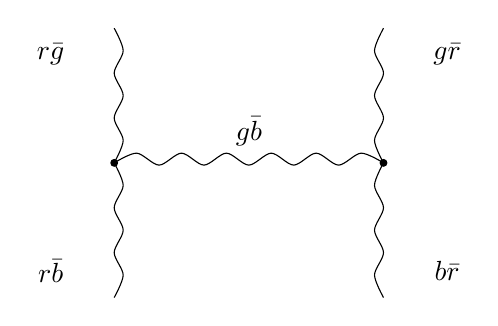
\begin{tikzpicture}[scale=0.95]
\draw[smooth] plot coordinates {
(-1.8,-1.8) (-1.68,-1.50) (-1.80,-1.20) (-1.68,-0.90)
(-1.80,-0.60) (-1.68,-0.30) (-1.8,0)
};
\draw[smooth] plot coordinates {
(-1.8,0) (-1.68,0.30) (-1.80,0.60) (-1.68,0.90)
(-1.80,1.20) (-1.68,1.50) (-1.8,1.8)
};
\draw[smooth] plot coordinates {
(1.8,-1.8) (1.68,-1.50) (1.80,-1.20) (1.68,-0.90)
(1.80,-0.60) (1.68,-0.30) (1.8,0)
};
\draw[smooth] plot coordinates {
(1.8,0) (1.68,0.30) (1.80,0.60) (1.68,0.90)
(1.80,1.20) (1.68,1.50) (1.8,1.8)
};
\draw[smooth] plot coordinates {
(-1.8,0) (-1.50,0.13) (-1.20,-0.03) (-0.90,0.13)
(-0.60,-0.03) (-0.30,0.13) (0,-0.03)
(0.30,0.13) (0.60,-0.03) (0.90,0.13)
(1.20,-0.03) (1.50,0.13) (1.8,0)
};
\node at (-2.65,-1.45) {$r\bar b$};
\node at (-2.65,1.45) {$r\bar g$};
\node at (2.65,-1.45) {$b\bar r$};
\node at (2.65,1.45) {$g\bar r$};
\node at (0,0.42) {$g\bar b$};
\fill (-1.8,0) circle (1.5pt);
\fill (1.8,0) circle (1.5pt);
\end{tikzpicture}
\caption{Обмен глюоном \(g\bar b\) между двумя глюонами, при котором каждая цветовая и антицветовая линия непрерывно проходит через вершины.}
\end{figure}

\section{Самодействие глюонов и нелинейные поля}

Самодействие глюонов меняет характер КХД. Кварки могут связываться, обмениваясь глюонами, и образовывать адроны, но и глюоны могут связываться, обмениваясь глюонами. Поэтому КХД может содержать составные объекты, целиком состоящие из глюонных степеней свободы, без кварков. В КЭД нет соответствующего элементарного связанного состояния, состоящего только из фотонов.

Язык полей приводит к тому же выводу. Две электромагнитные волны в пустом пространстве проходят друг сквозь друга на элементарном уровне. Две глюонные волны взаимодействуют и деформируют друг друга. Даже разные части одной конфигурации глюонного поля могут действовать друг на друга силами. Поэтому глюонное поле нелинейно.

\begin{classroomqa}
\audiencequestion{Должно ли по обе стороны диаграммы появляться одинаковое число красных, зелёных и синих меток?\lecturetimestamp{01:24:59}}
\lecturerresponse{Практическое правило состоит в том, чтобы прослеживать каждую цветовую линию по диаграмме. Эта непрерывность и есть сохранение цвета. Если фермионная линия разворачивается по времени, её метка становится соответствующей меткой античастицы или антицвета.}
\end{classroomqa}

\begin{classroomqa}
\audiencequestion{Согласованы ли все цветовые и антицветовые метки в первой версии диаграммы?\lecturetimestamp{01:26:00}}
\lecturerresponse{Нет. Несколько меток нужно исправить. В согласованном назначении красная, антисиняя и зелёная линии каждая продолжается через вершины, а обращённая фермионная стрелка интерпретируется как античастица.}
\end{classroomqa}

\begin{classroomqa}
\audiencequestion{Рассматривается ли промежуточная глюонная линия как пара кварк--антикварк?\lecturetimestamp{01:27:58}}
\lecturerresponse{Только в цветовом учёте. Глюон не является буквально композитом кварк--антикварк, но он несёт соответствующие свойства цвета и антицвета.}
\end{classroomqa}

На этом этапе элементарные правила можно сформулировать кратко:

\begin{itemize}
\item кварки испускают и поглощают глюоны;
\item глюоны непосредственно взаимодействуют с глюонами;
\item каждая цветовая и антицветовая линия должна продолжаться через вершину;
\item обращение фермионной линии по времени превращает её в соответствующую линию античастицы.
\end{itemize}

\begin{classroomqa}
\audiencequestion{Остаются ли глюоны безмассовыми, когда их представляют всеми этими линиями цвет--антицвет?\lecturetimestamp{01:28:13}}
\lecturerresponse{Да. Глюоны остаются безмассовыми. Следующее уточнение касается того, что имеется в виду под массой, приписываемой кварку внутри адрона.}
\end{classroomqa}

Далее идут конфайнмент и структура адронов: почему изолированный цвет никогда не наблюдается и как кварки и глюоны организуются внутри составных частиц. Сначала полезно уточнить, что имеется в виду под массой конституэнтного кварка.

\section{Масштаб зондирования и смысл массы кварка}

Представьте себе маленький объект массы \(m\), прикреплённый к мягкому деформируемому куску материала---подойдёт свисающий кусочек жевательной резинки. Приложите очень слабую силу, настолько медленно, что мягкий материал успевает приспособиться и вся система движется вместе. Тогда измеряемая инерция есть инерция маленького объекта плюс присоединённого материала.

Теперь заставьте маленький объект колебаться с очень высокой частотой. Мягкий материал не успевает следовать за быстрым движением. Он остаётся почти неподвижным, тогда как откликается малое ядро. Тогда измеряемая высокочастотная инерция оказывается гораздо ближе к одному лишь \(m\).

\begin{figure}[h]
\centering
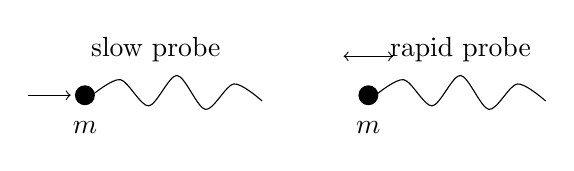
\begin{tikzpicture}[scale=0.9]
\fill (-3,0) circle (4pt);
\node at (-3,-0.45) {$m$};
\draw[smooth] plot coordinates {
(-2.9,0) (-2.5,0.22) (-2.1,-0.15) (-1.7,0.28)
(-1.3,-0.20) (-0.9,0.16) (-0.5,-0.08)
};
\draw[->] (-3.8,0) -- (-3.2,0);
\node at (-2.0,0.65) {slow probe};

\fill (1.0,0) circle (4pt);
\node at (1.0,-0.45) {$m$};
\draw[smooth] plot coordinates {
(1.1,0) (1.5,0.22) (1.9,-0.15) (2.3,0.28)
(2.7,-0.20) (3.1,0.16) (3.5,-0.08)
};
\draw[<->] (0.65,0.55) -- (1.35,0.55);
\node at (2.3,0.65) {rapid probe};
\end{tikzpicture}
\caption{Медленное зондирование перемещает ядро и его мягкую оболочку вместе, тогда как быстрое зондирование сначала измеряет главным образом отклик самого ядра.}
\end{figure}

Это классическая аналогия. Определяемая масса зависит от частоты приложенной силы, потому что при разных частотах разные части системы успевают участвовать.

Кварк внутри адрона окружён сильно взаимодействующим глюонным веществом и другими составляющими. Если бы можно было тянуть кварк очень медленно, откликался бы весь адрон. Тогда ощущаемая инерция была бы порядка массы нуклона,
\begin{equation}
m_N\sim930\text{--}940\,\mathrm{MeV}.
\end{equation}
Если же по кварку нанести очень сильный удар и зондировать его в течение очень короткого времени, начальный отклик связан с гораздо меньшим параметром массы, который по соглашению приписывают лёгкому кварку, примерно
\begin{equation}
m_{u,d}\sim5\text{--}10\,\mathrm{MeV}
\end{equation}
в используемых здесь оценках.

Таким образом, выражение ``масса кварка'' требует указания масштаба зондирования. Мягкое низкочастотное возмущение приводит в движение протяжённый составной объект; жёсткое высокочастотное возмущение сначала разрешает гораздо меньшую его часть. Эта аналогия не является выводом перенормировки, но она помогает понять, почему параметры, используемые для описания частиц, зависят от частот и длин волн взаимодействий, в которых они измеряются. Такие зависящие от масштаба параметры называются бегущими параметрами или бегущими константами.

\begin{classroomqa}
\audiencequestion{Является ли эта зависящая от частоты масса лишь переформулировкой соотношения неопределённостей, такого как \(\Delta x\,\Delta t\)?\lecturetimestamp{01:33:32}}
\lecturerresponse{Нет. Этот пример уже носит классический характер. Небольшая масса, прикреплённая к чему-то мягкому, ускоряется одним образом под действием быстрой силы и другим под действием медленной силы, потому что откликнуться успевают разные доли присоединённого материала.}
\end{classroomqa}

\begin{classroomqa}
\audiencequestion{Проявляется ли в предыдущем обсуждении электрического заряда электрона та же зависимость от масштаба?\lecturetimestamp{01:34:04}}
\lecturerresponse{Да. Общий вывод состоит в том, что параметры, используемые для описания частиц, зависят от частот и длин волн взаимодействий, с помощью которых их зондируют. Их называют бегущими константами.}
\end{classroomqa}

\begin{classroomqa}
\audiencequestion{Применима ли та же оговорка к дробному заряду, приписываемому кварку?\lecturetimestamp{01:34:36}}
\lecturerresponse{Да. Нужно тщательно определить, что имеется в виду под зарядом кварка. На этом уровне его указывают относительно заряда протона; более полное определение — тема отдельного обсуждения.}
\end{classroomqa}

\editorialnote{Фиксированное дробное квантовое число электрического заряда и зависящая от масштаба константа связи взаимодействия — разные вещи. Бег константы связи не изменяет сами метки аромата \(+\tfrac23\) или \(-\tfrac13\).}

\begin{classroomqa}
\audiencequestion{Почему при учете цвета всегда используют кварк и антикварк? Почему соответствующий объект не могли бы образовать два кварка?\lecturetimestamp{01:34:55}}
\lecturerresponse{Это важный вопрос, но ответ на него относится к следующему обсуждению допустимых цветовых комбинаций и конфайнмента.}
\end{classroomqa}

\begin{classroomqa}
\audiencequestion{Если отдельные кварки нельзя изолировать, то как были сделаны выводы о дробном заряде, цвете и кварковой модели?\lecturetimestamp{01:35:17}}
\lecturerresponse{Эта картина складывалась постепенно из множества свидетельств наряду с кажущимися противоречиями. Закономерности в мире адронов указывали на кварковые составляющие; состояния Delta выявили конфликт со статистикой Ферми; а постоянный конфайнмент кварков оказался еще одним необычным фактом. Кварковая гипотеза появилась в начале 1960-х годов, Nambu принадлежала важная ранняя версия идеи цвета, а многие физики на протяжении примерно следующего десятилетия собирали полную структуру воедино и проверяли ее. Это не было результатом одного наблюдения или труда одного человека.}
\end{classroomqa}

\begin{classroomqa}
\audiencequestion{Почему существует только 8 глюонов, а не 9 очевидных комбинаций цвет--антицвет?\lecturetimestamp{01:37:24}}
\lecturerresponse{Подробное объяснение того, почему диагональная сумма не является дополнительным глюоном, отложено.}
\end{classroomqa}

\begin{classroomqa}
\audiencequestion{Игнорируются ли в этом обсуждении КХД электроны?\lecturetimestamp{01:37:33}}
\lecturerresponse{Да. КХД выделяется точно так же, как при обсуждении КЭД можно временно не учитывать кварки. Эти отдельные секторы в конечном счете нужно объединить в более крупную структуру, включающую кварки, электроны, фотоны и другие частицы. Некоторые части этого более широкого синтеза уже осуществлены, а некоторые остаются незавершенными. В физике часто действуют так: выделяют подсистему, понимают ее, а затем снова собирают части воедино.}
\end{classroomqa}